\documentclass{article}

\usepackage{fancyhdr} % Required for custom headers
\usepackage{lastpage} % Required to determine the last page for the footer
\usepackage{extramarks} % Required for headers and footers
\usepackage[usenames,dvipsnames]{color} % Required for custom colors
\usepackage{graphicx} % Required to insert images
\usepackage{listings} % Required for insertion of code
\usepackage{courier} % Required for the courier font
\usepackage{caption}
\usepackage{subcaption}
\renewcommand{\_}{\char`_}

% Margins
\topmargin=-0.45in
\evensidemargin=0in
\oddsidemargin=0in
\textwidth=6.5in
\textheight=9.0in
\headsep=0.25in

\linespread{1.1} % Line spacing

\lstset{language=C,
                basicstyle=\ttfamily,
                keywordstyle=\color{blue}\ttfamily,
                stringstyle=\color{red}\ttfamily,
                commentstyle=\color{Plum}\ttfamily,
                morecomment=[l][\color{magenta}]{\#}
}


% Set up the header and footer
\pagestyle{fancy}
\lhead{Group 18} % Top left header
\chead{Task 0: Alarm Clock} % Top center head
\rhead{\firstxmark} % Top right header
\lfoot{\lastxmark} % Bottom left footer
\rfoot{Page\ \thepage\ of\ \protect\pageref{LastPage}} % Bottom right footer
\renewcommand\headrulewidth{0.4pt} % Size of the header rule
\renewcommand\footrulewidth{0.4pt} % Size of the footer rule

\setlength\parindent{0pt} % Removes all indentation from paragraphs

%----------------------------------------------------------------------------------------
%	TITLE PAGE
%----------------------------------------------------------------------------------------

\title{
\vspace{2in}
\textmd{\textbf{Task 1: Scheduling}}\\
\normalsize\vspace{0.1in}\small{Due\ on\ Tuesday,\ February\ 9,\ 2016}\\
\vspace{0.1in}\large{\textbf{Pintos Group 18}}
\vspace{3in}
}

\author{Corentin Herbinet, Ignacio Navarro, Vinothan Shankar, William Springsteen}
\date{}

%----------------------------------------------------------------------------------------

\begin{document}

\maketitle
\newpage

\section{Design Questions: Priority Scheduling}
\subsection{Data Structures}
\subsubsection{Purpose of new variables}

\begin{enumerate}

\item \begin{lstlisting}
struct thread
  {
		.
		.
    struct list locks_holding;           /* List of locks that thread owns. */
    struct lock *waiting_on_lock; 	 /* Lock the thread is waiting on. */ 
    struct semaphore *waiting_on_sema;   /* Semaphore the thread is waiting on. */
		.
		.
  };
\end{lstlisting}

\item \begin{lstlisting}
struct lock 
  {
    struct thread *holder;       /* Thread holding lock (for debugging). */
    struct list_elem lock_elem;  /* For the list of locks a thread has.  */
    struct semaphore semaphore;  /* Binary semaphore controlling access. */
  };
\end{lstlisting}
\end{enumerate}


\begin{enumerate}

\item We have modified \texttt{struct thread} by adding three new members. The first is a list of locks that the thread owns. This 
is useful to modify the effective priority. The second is a pointer to a lock that the thread is waiting on. This pointer is \texttt{NULL}
if the thread is not waiting on any lock. This member is useful to donate priority along the chain. The third is another pointer to a semaphore. This is used in the same manner as the second member but with semaphores, since a thread could be waiting on a semaphore but not on a lock.

\item We have modified only one member in \texttt{struct lock}. This is a \texttt{list\_elem} for the list of locks a thread owns, as explained
in the previous part.
\end{enumerate}

\subsubsection{Data structure used to track priority donation}
To track priority donation we've added a list \texttt{locks\_holding} that each thread has, a lock \texttt{waiting\_on\_lock} that each thread is waiting on (if a thread is not waiting, then this is set to \texttt{NULL}), and a thread \texttt{holder} that each lock has. This is sufficient to track priority donation by the following means. We use two functions \texttt{thread\_donate\_priority(struct thread *donee, int priority)} and \\ \texttt{thread\_recalculate\_priority(struct thread *t)}. The donate function works recursively by donating priority to lower priority threads that have locks a higher priority thread needs access to. Say thread A with higher priority than thread B wants to acquire a lock that thread B owns. Hence in this case the lock's \texttt{holder} would be B, and thread A would set \texttt{waiting\_on\_lock} to point to the lock. Now since A is stuck waiting on thread B, it calls \texttt{lock\_acquire()}, which calls \texttt{sema\_down()}, which itself calls the function \texttt{thread\_donate\_priority(B, A->effective\_priority)}. This function would allow B to have enough priority to run, call \texttt{lock\_release()} to release the lock, and allow A to acquire the lock. When B releases the lock, it calls  \texttt{thread\_recalculate\_priority(B)} which searches through \texttt{locks\_holding} to recalculate the effective priority back so that B, having originally a lower priority, doesn't run. The next example of nested priorities should give a more intuitive feel of how the system works.
\newpage

\begin{figure}[ht!]
\centering
\hspace{3em}
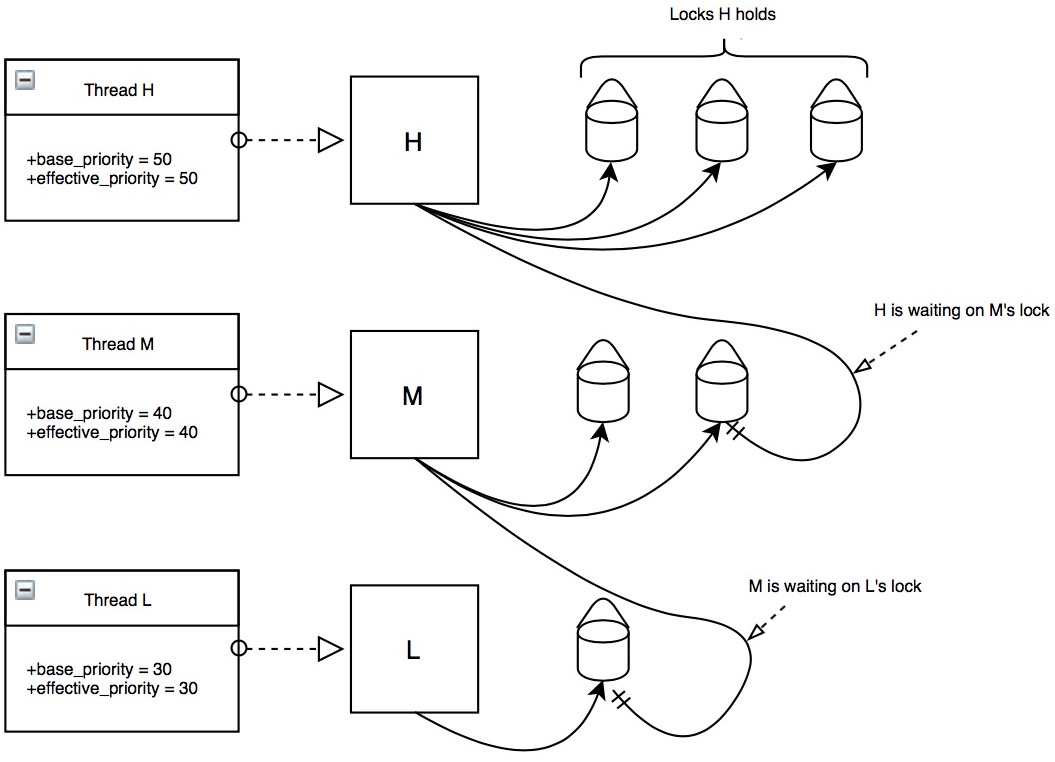
\includegraphics[width=0.6\textwidth]{Images/Task1/1Nested}
\caption{Initial State}
\end{figure}

In the following scenario (Figure 1), thread H is the highest priority thread and therefore in the running state. It currently has three locks, and wants to acquire a fourth by calling \texttt{lock\_acquire()}. If no thread owns the lock (i.e. \texttt{holder} is \texttt{NULL}), then H can acquire the lock. 

\begin{figure}[ht!]
\centering
\hspace{3em}
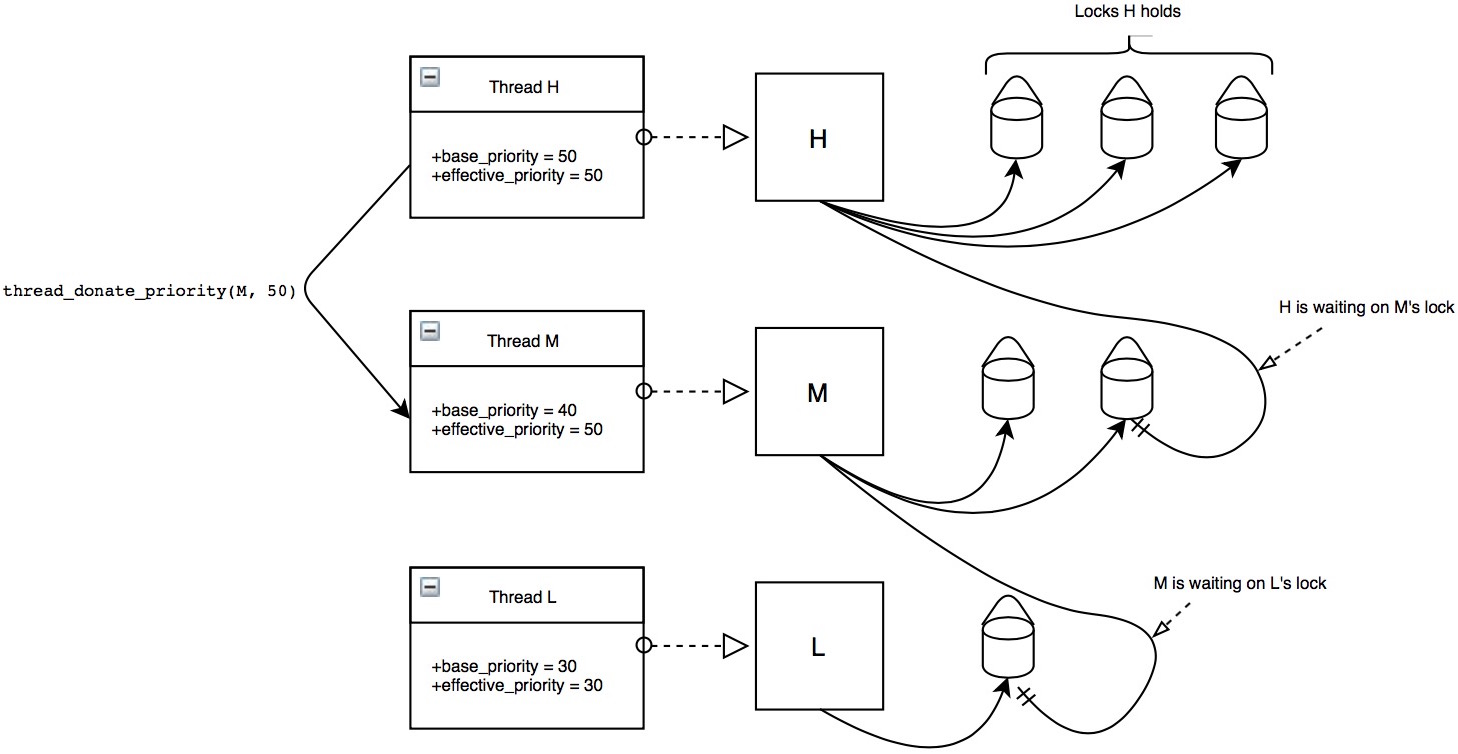
\includegraphics[width=0.8\textwidth]{Images/Task1/2Nested}
\caption{Second State}
\end{figure}

However, M has the lock, so H calls \texttt{thread\_donate\_priority(M, H->effective\_priority)} in Figure 2 so that M can release the lock, recalculate its priority, and H can continue to run. Unfortunately, it is the case that M itself is waiting on another lock L has, so M calls recursively \texttt{thread\_donate\_priority(L, M->effective\_priority)}, as shown in Figure 3.
\newpage

\begin{figure}[ht!]
\centering
\hspace{3em}
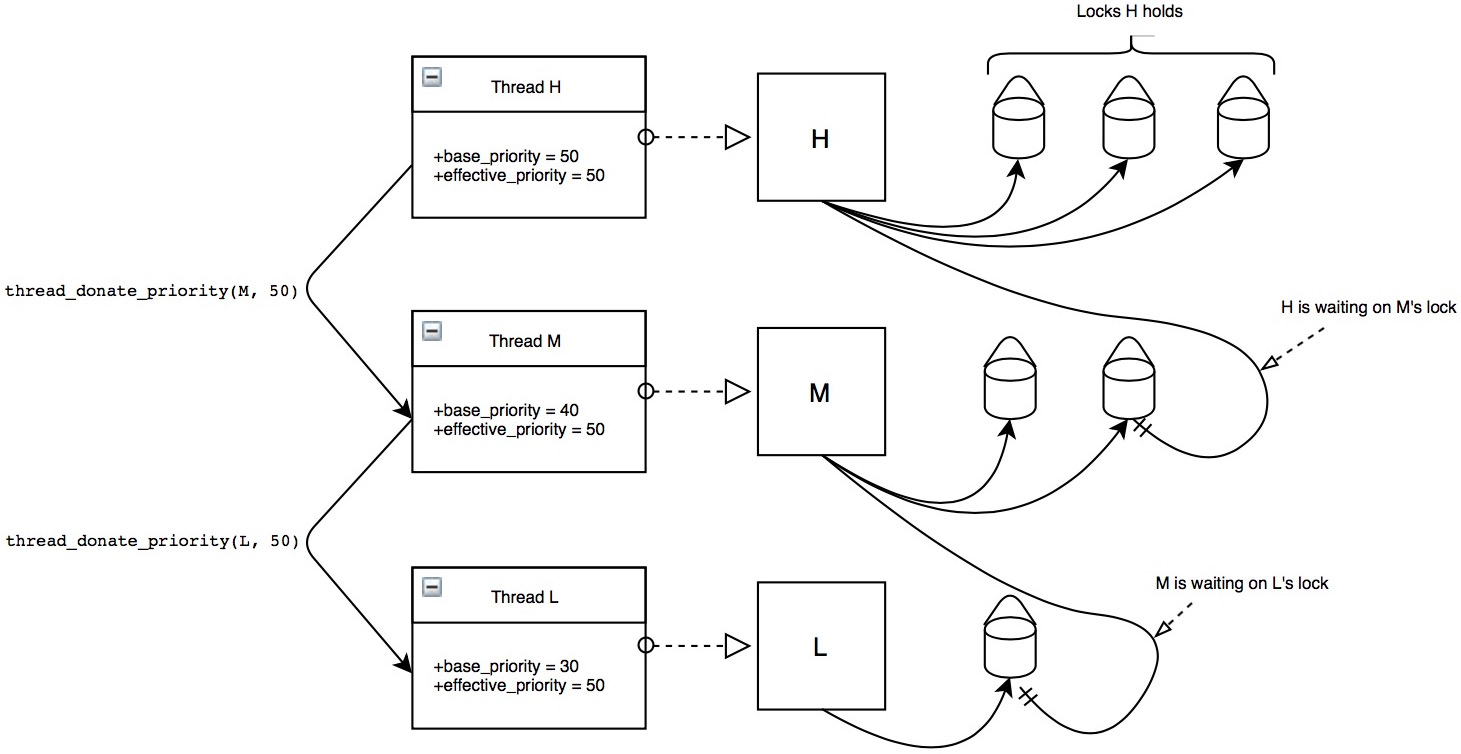
\includegraphics[width=0.8\textwidth]{Images/Task1/3Nested}
\caption{Third State}
\end{figure}

Now L has effective priority 50 and therefore runs. It checks if it is waiting on a lock through \texttt{waiting\_on\_lock}, (it isn't), so we have reached a base case, and \texttt{thread\_donate\_priority(L, M->effective\_priority)} simply returns. L continues to run, and releases the lock it's holding through \texttt{lock\_release()}. This in turn calls \texttt{thread\_recalculate\_priority(L)}, which checks the list of locks L holds \texttt{locks\_holding}. We iterate through all the locks L holds and see for each lock the list of waiting threads on that lock. The highest priority waiting thread would then set the effective priority of L to its effective priority. However, since L is not holding any locks, we simply set the effective priority to the base priority (Figure 4). 

\begin{figure}[ht!]
\centering
\hspace{3em}
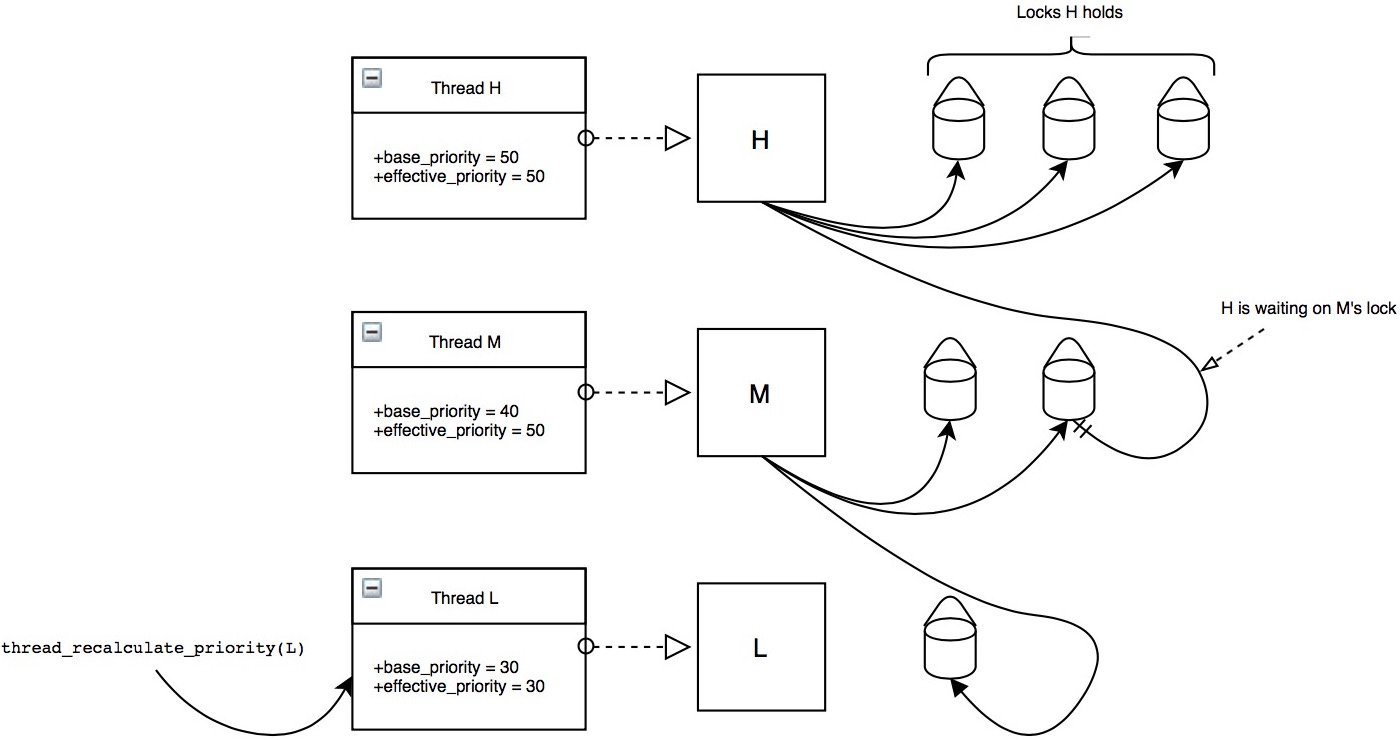
\includegraphics[width=0.8\textwidth]{Images/Task1/4Nested}
\caption{Fourth State}
\end{figure}

Note that in Figure 4 thread L has released the lock, and M is therefore not waiting on any more locks. It would therefore be unblocked and put in a running state. Since M is now running, it can release the lock H wants through \texttt{lock\_release()} which in turn calls \texttt{thread\_recalculate\_priority(M)}. We again iterate through all the locks M holds and see for each lock the list of waiting threads on that lock. The highest priority waiting thread would then set the effective priority of M to its effective priority. However, since M's list of locks have no waiters, we simply set the effective priority to the base priority (Figure 5). 

\begin{figure}[ht!]
\centering
\hspace{3em}
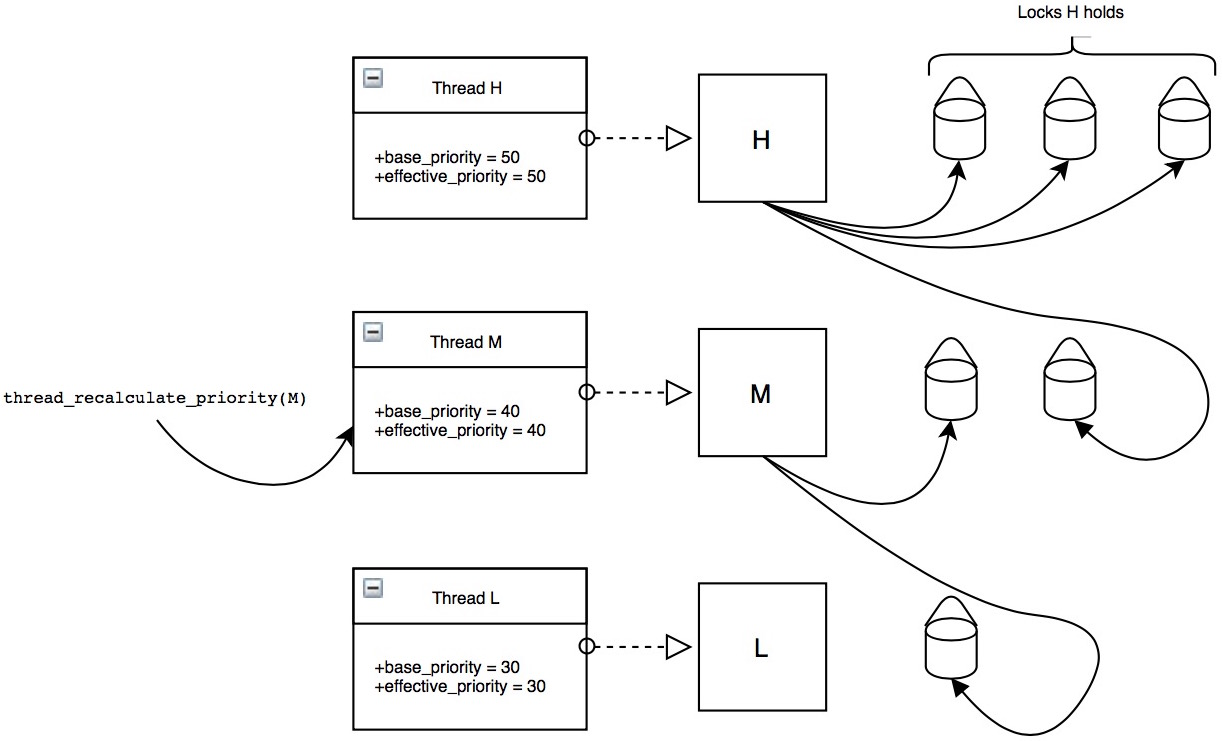
\includegraphics[width=0.8\textwidth]{Images/Task1/5Nested}
\caption{Fifth State}
\end{figure}

Again note how now M has released the lock and set back its effective priority.

\begin{figure}[ht!]
\centering
\hspace{3em}
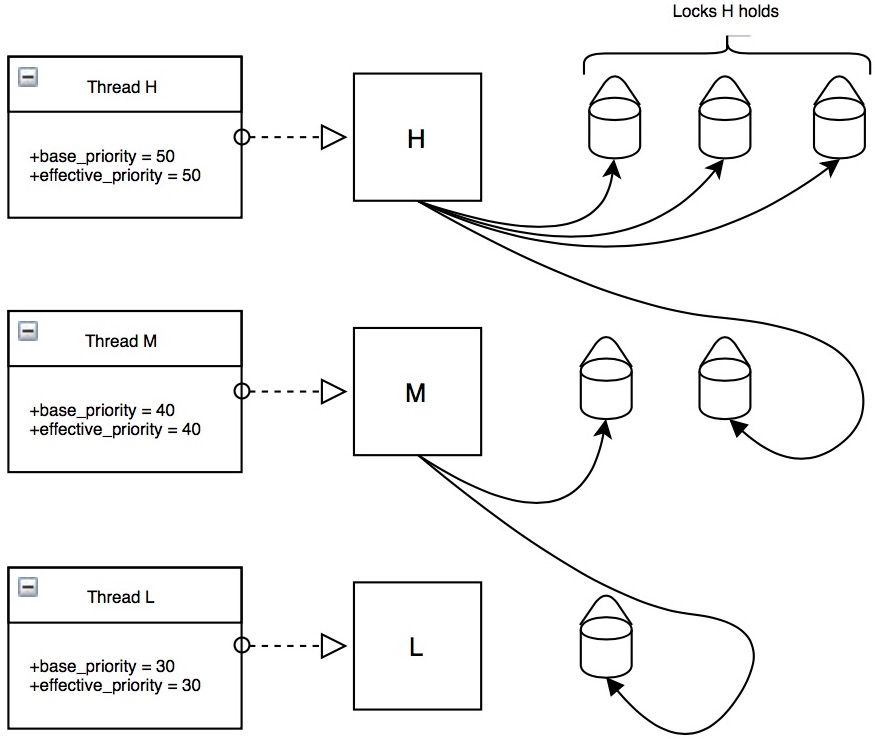
\includegraphics[width=0.6\textwidth]{Images/Task1/6Nested}
\caption{Final State}
\end{figure}

We thus reach our final state, avoiding starvation and deadlock.


%\begin{figure*}
%    \centering
%    \begin{subfigure}[b]{0.50\textwidth}
%   	    \hspace{2em}
%            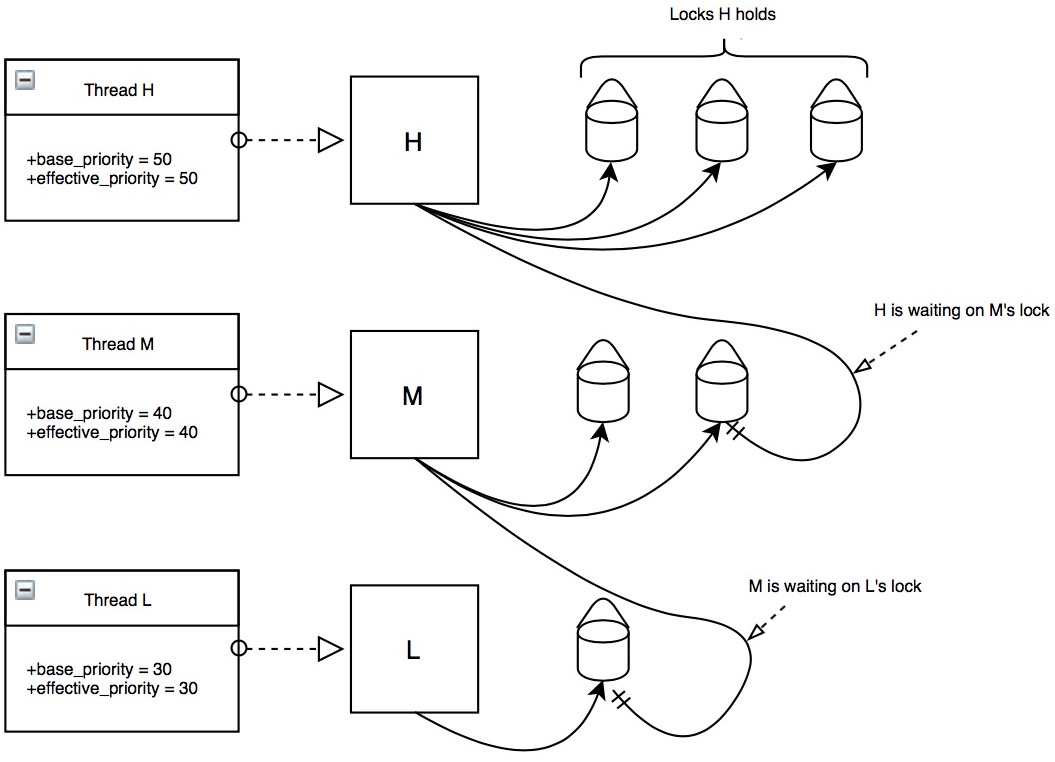
\includegraphics[width=\textwidth]{Images/Task1/1Nested}
%            \caption{Initial State}
%            \label{fig:a}
%    \end{subfigure}
%    
%    \begin{subfigure}[b]{0.49\textwidth}
%            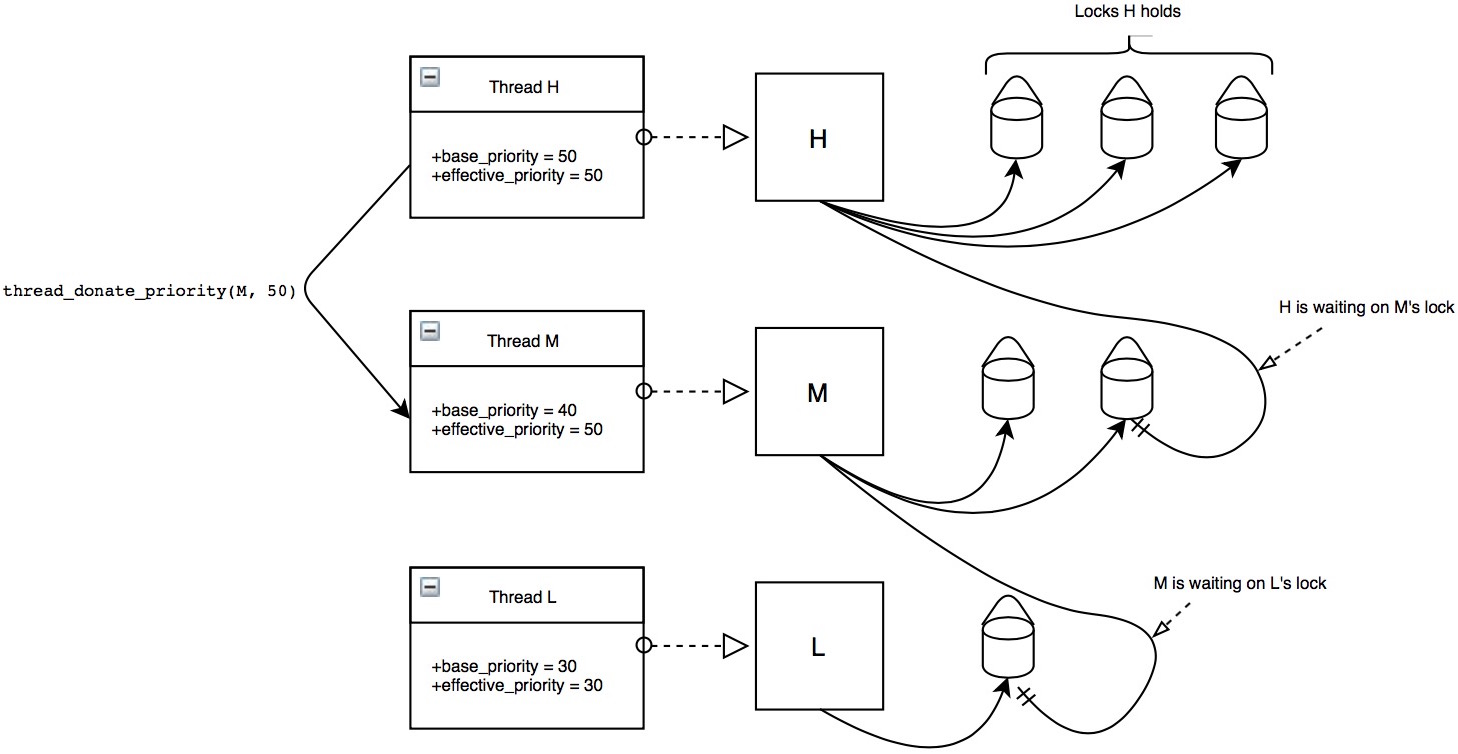
\includegraphics[width=\textwidth]{Images/Task1/2Nested}
%            \caption{c}
%            \label{fig:c}
%    \end{subfigure}
%    % ... this comment too
%    \begin{subfigure}[b]{0.49\textwidth}
%            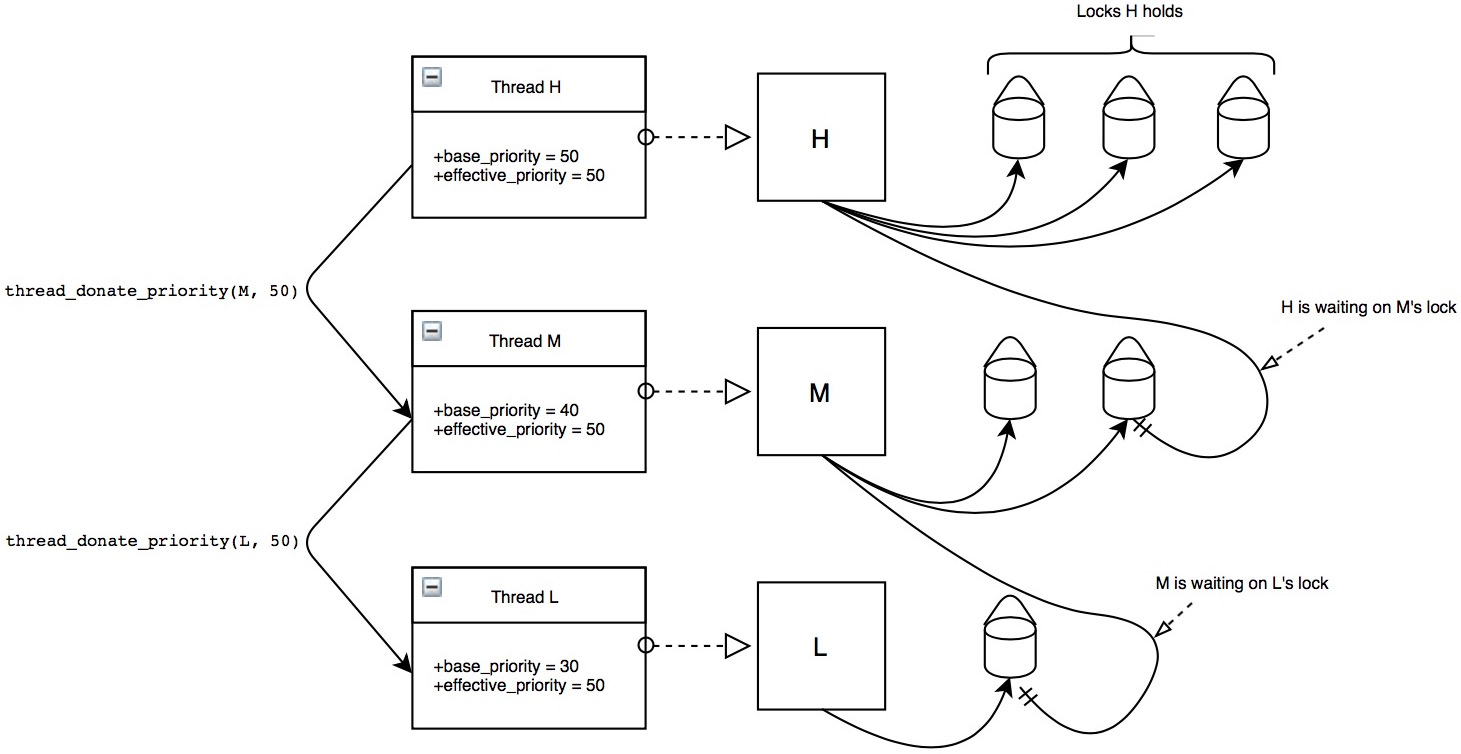
\includegraphics[width=\textwidth]{Images/Task1/3Nested}
%            \caption{d}
%            \label{fig:d}
%    \end{subfigure}
%    \begin{subfigure}[b]{0.49\textwidth}
%            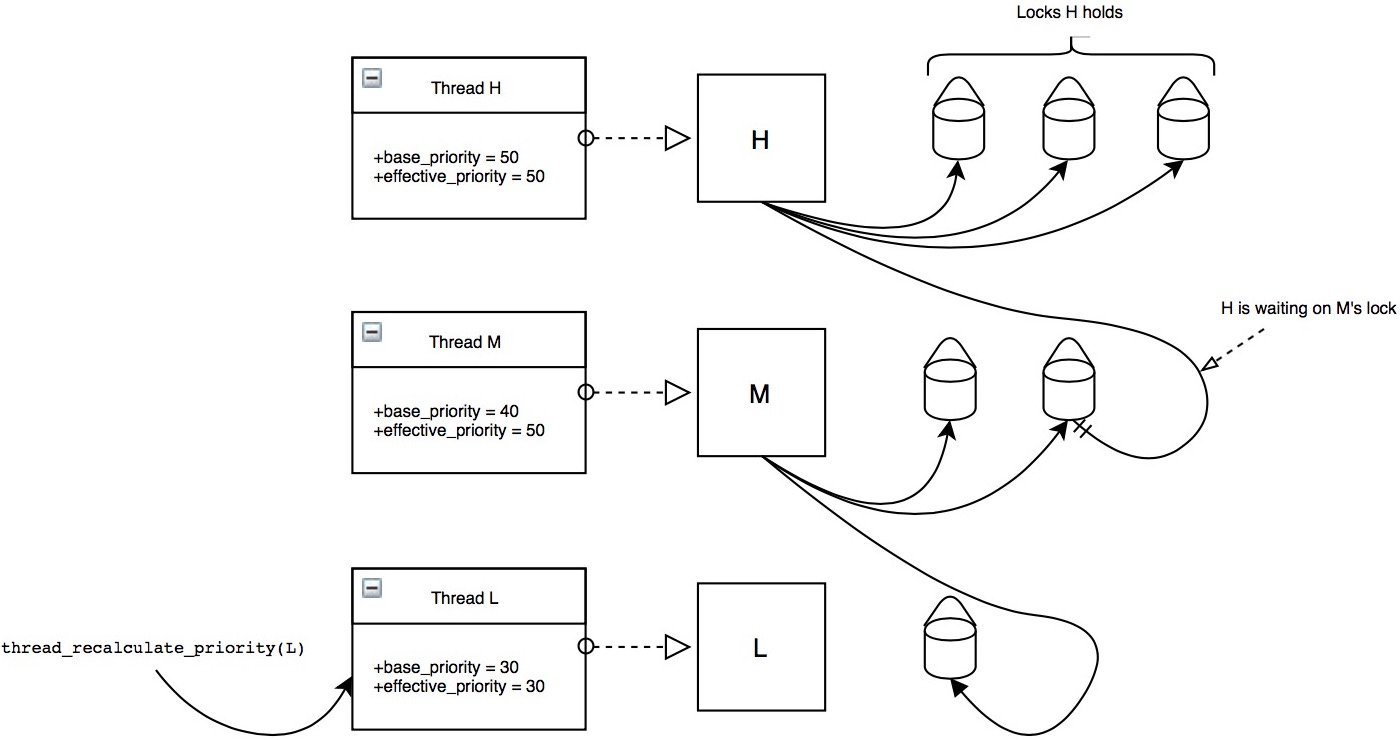
\includegraphics[width=\textwidth]{Images/Task1/4Nested}
%            \caption{c}
%            \label{fig:c}
%    \end{subfigure}
%    % ... this comment too
%    \begin{subfigure}[b]{0.49\textwidth}
%            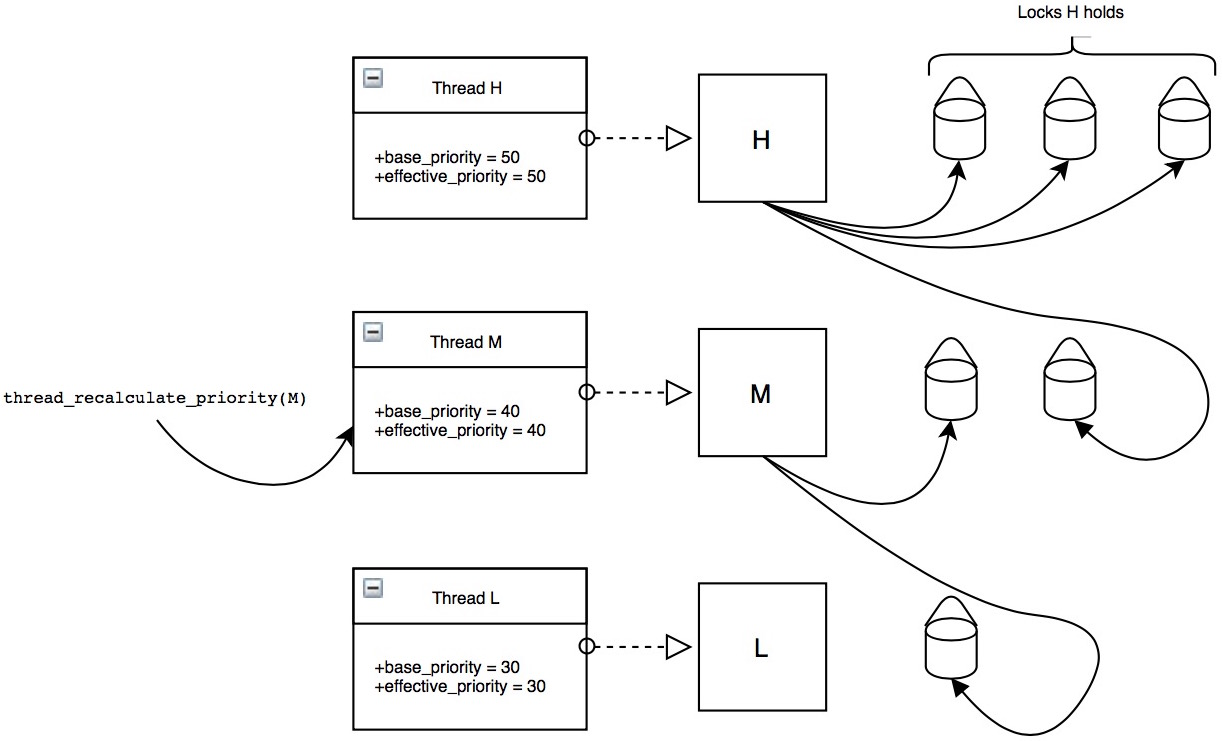
\includegraphics[width=\textwidth]{Images/Task1/5Nested}
%            \caption{d}
%            \label{fig:d}
%    \end{subfigure}
%     \begin{subfigure}[b]{0.50\textwidth}
%            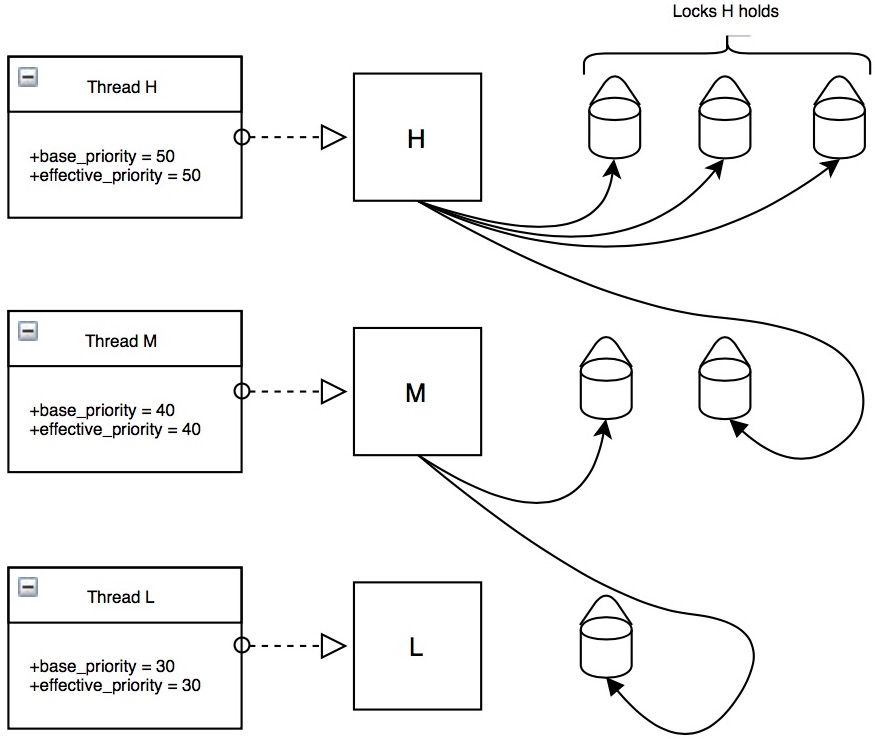
\includegraphics[width=\textwidth]{Images/Task1/6Nested}
%            \caption{Initial State}
%            \label{fig:a}
%    \end{subfigure}
%    \caption{Pictures of ABCD}\label{fig:ABCD}
%\end{figure*}


\subsection{Algorithms}
\subsubsection{Ensuring highest priority thread wakes up first}

\subsubsection{Sequence of events in \texttt{lock\_acquire()}}

\subsubsection{Sequence of events in \texttt{lock\_release()}}

\subsection{Synchronization}
\subsubsection{Potential race in \texttt{thread\_set\_priority()}}

\subsection{Rationale}

\subsubsection{Choice of design and superiority to other designs}

\newpage

\section{Design Questions: Advanced Scheduler}
\subsection{Data Structures}
\subsubsection{Purpose of new variables}

\subsection{Algorithms}
\subsubsection{Table}
\subsection{Ambiguities in scheduler specification and resolution}
\subsubsection{Dividing cost of scheduling}

\subsection{Rationale}
\subsubsection{Critique of design}

\subsubsection{Design in fixed-point arithmetic}


%----------------------------------------------------------------------------------------

\end{document}